\chapter{RPC - Remote Procedure Call}
\section{Definizione}
L'RPC p un meccanismo progettato per permettere ai programmi di invocare procedure (funzioni o metodi) \textbf{\uline{che si trovano fisicamente su macchine remote}}.

A differenza dei tradizionali approcci basati sullo scambio esplicito di messaggi dove il programmatore deve gestire e scrivere attivamente il codice per la comunicazione di rete, \textbf{l'obiettivo fondamentale di RPC} \uline{è garantire la trasparenza}, questo significa che \uline{il programmatore effettua la chiamata nel codice esattamente nel solito modo in cui chiamerebbe una funzione locale}, nascondendo quasi del tutto l'esistenza di una rete.

\begin{figure}[H]
    \centering
    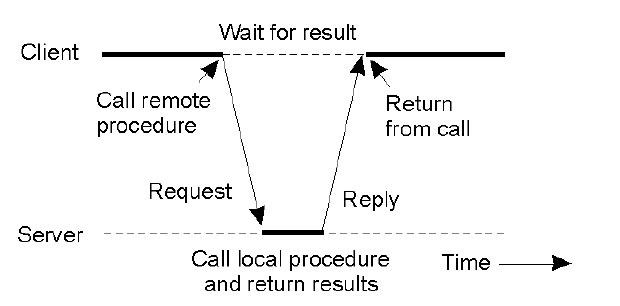
\includegraphics[scale=0.65]{figures/Schermata_20260514_112551.png}
\end{figure}

\section{Architettura RPC}
La scopo principale dell'Architettura RPC è mascherare la comunicazione di rete e far apparire l'invocazione di una funzione remota esattamente come se fosse una chiamata locale.

Per ottenere questa "trasparenza", l'architettura RPC delega tutta la complessità della comunicazione a un middleware composto da due elementi speculari, chiamti \textbf{stub} (o proxy/skeleton)
\subsection{Client stub (o proxy)}
È un oggetto che risiede sulla macchina del client e che offre al programma chiamante la stessa identica interfaccia della procedura remota, quando il programma effettua la chiamata, in realtà sta invocando il client stub.

Il compito di questo componente è raccogliere i parametri forniti, impacchettarli in un messaggio, spedire la richiesta attraverso la rete e sospendere l'esecuzione in attesa.

Quando arriva la risposta del server, estrae il risultato e lo restituisce al chiamante, simulando la presenza locale della risorsa.
\subsection{Server Stub (o skeleton)}
Risiede sulla macchina del server.

Il suo ruolo è rimanere in ascolto, ricevere il messaggio di rete inviato dal client, decompacchettarlo per estrarre i parametri originali e invocare la vera procedura locale.

Una volta terminata l'elaborazione, il server stub raccoglie il risultato, crea un messaggio di risposta e lo invia indietro al client.

\section{Procedura generale e il ruolo del Middleware}
Quando un programma sul client invoca una procedura remota, la sua esecuzione viene momentaneamente bloccata.

La chiamata viene intercettata da un software intermedio, chiamato \textbf{middleware} che \uline{si occupa di tradurre la chiamata locale in un pacchetto di richiesta}, lo spedisce al server e rimane in attesa.

Quando il server remoto termina l'esecuzione e restituisce la risposta, \uline{il middleware lo scompatta e la consegna al programma chiamante}, che a quel punto sblocca la sua esecuzione e procede.

In questo modo l'RPC riesce a \textbf{"mascherare"} il modello client-server.

\subsection{Vantaggi e Svantaggi}
\subsubsection{Vantaggi}
\textbf{È molto intuitiva} perchè \uline{utilizza una semantica bene nota} a tutti i programmari e \uline{si adatta perfettamente alle architetture clien-server}.
\subsubsection{Svantaggi}
Poichè la procedura viene eseguita su una macchina diversa da quella chiamante, i due processi vivono in \textbf{spazi di indirimzzamento della memoria differenti}.

Questo rende il \uline{passaggio dei parametri e dei risultati molto complesso da gestire}, soprattutto perchè gli indirizzi di memoria hanno valenza puramente locale e non hanno alcun senso se spediti a un computer diverso.


\section{Passaggio dei parametri}
Il problema del passaggio dei parametri in una RPC nasce dal fatto che il processo chiamante (client) e il processo chiamato (server) vengono eseguiti su macchine fisicamente distinte e, di conseguenza, si trovano in spazi di indirizzamento della memoria differenti.

Nelle chiamate di procedura convnzionali (locali), i parametri possono essere passati attraverso due logiche principali:
\begin{itemize}
    \item \textbf{Per valore (call-by-value)}

    Viene passata solo una copia del dato, eventuali modifiche effettuate dalla procedura chiamata non intaccano la variabile originale del chiamante.
    \item \textbf{Per riferimento (call-by-reference)}
    
    Viene passato l'indirizzo di memoria (un puntatore) in cui si trova il dato.

    In questo caso, la procedura lavora direttamente sull'oggetto originale e le sue modifiche sono visibili al chiamante.
\end{itemize}

In un sistema basato su RPC, \textbf{l'approccio del passaggio per riferimento è problematico e inapplicabile direttamente.}

Gli indirizzi di memoria hanno infatti una valenza strettamente locale: inviare un puntatore della RAM del client al server non ha alcun senso, in quanto quell'indirizzo non corrisponderà alla stessa risorsa sulla macchina di destinazione.

\subsection{Meccanismo call-by-copy/restore}
Per aggirare l'ostacolo dell'approccio per passaggio di riferimento, si utilizza un meccanismo chiamato \textbf{call-by-copy/restore}, questo approccio si divide in 4 fasi:
\begin{enumerate}
    \item Al momento della chiamata, il client \uline{copia il valore corrente della variabile (nello stack)} e lo spedisce al server attraverso la rete.
    \item Il server riceve i dati e la procedura remota esegue le sue operazioni lavorando sulla copia appena ricevuta.
    \item Terminata l'elaborazione, il dato modificato dal server \uline{viene impacchettato e inviato nuovamente indietro} nella risposta.
    \item Il client riceve la risposta e \textbf{sovrascrive la sua variabile originale locale} con la versione aggiornata restituita dal server.
    
    Grazie a questa sovrascrittura finale, l'effetto pratico sul client risulta \uline{totalmente analogo a quello di una chiamata per riferimento (call-by-reference)}, ma senza mai aver scambiato reali indirizzi di memoria.
\end{enumerate}

\begin{figure}[H]
    \centering
    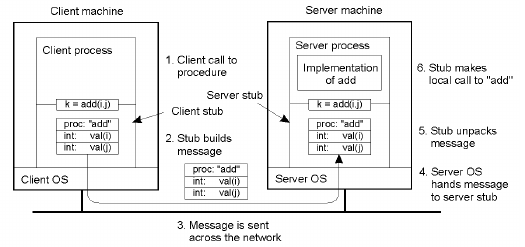
\includegraphics{figures/Schermata_20260514_141634.png}
\end{figure}

\section{Passaggio dei dati}
Poichè le strutture dati complesse non possono viaggiare "cosi' come sono" su un cavo di rete, gli stub devono trasformarle.

Per fare ciò si effettuano 2 passaggi.

\subsection{Serializzazione/Deserializzazione}
È la \uline{conversione delle strutture dai presenti nella memoria RAM in un formato} (come testo o sequenza di byte binari) \uline{adatto alla trasmissione sulla rete}.

L'operazione inversa per \uline{ricostruire il dato in memoria} si chiama \textbf{Deserializzazione}.

\subsection{Marshalling / Unmarshalling}
È il processo di \uline{impacchettamento vero e proprio dei dati serializzati} all'interno del messaggio di rete.

L'\textbf{unmarshalling} è \uline{l'operazione inversa di estrazione e scompattamento}.

Affichè il cient e server si capiscano senza errori durante queste operazioni di traduzione, il formato e la codifica dei dati devono essere rigorosamente condivisi tra i due stub.

Questo accordo viene tipicamente stabilito utilizzando dei linguaggi di definizione delle intergaccie (\texttt{IDL}), come ad esempio i file \texttt{ProtoBuf} usati nella moderna implementazione \texttt{gRPC}.

\begin{figure}[H]
    \centering
    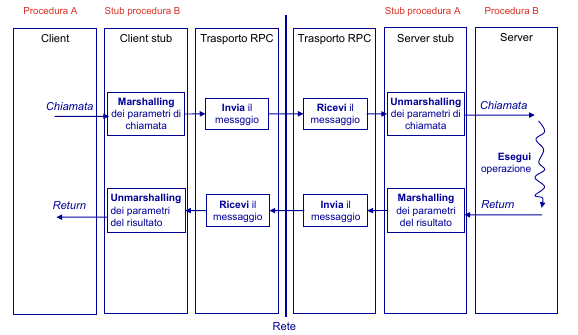
\includegraphics{figures/Schermata_20260515_103330.png}
    \caption{Esecuzione di una RPC}
\end{figure}

\chapter{gRPC}
\section{Definizione}
Sviluppato originariamente da Google nel 2015, è un framework \texttt{RPC} open source progettato per garantire \textbf{prestazioni elevatissime}.

A differenza di protocolli più lenti e pesanti

\section{Funzionalità di gRPC}
\subsection{Modelli di comunicazione}:
Permette quattro \textbf{modelli di comunicazione}:
\begin{enumerate}
    \item \textbf{Unary RPC}: Classico schema richiesta-risposta.
    \item \textbf{Server Streaming}: Il client invia una richiesta e il server risponde con un flusso continuo di messaggi.
    \item \textbf{Client Streaming}: Il client invia un flusso di messaggi e il server risponde una volta solo alla fine.
    \item \textbf{Bidirectional Streaming}: Entrambi inviano flussi di messaggi simultaneamente.
\end{enumerate}

\begin{figure}[H]
    \centering
    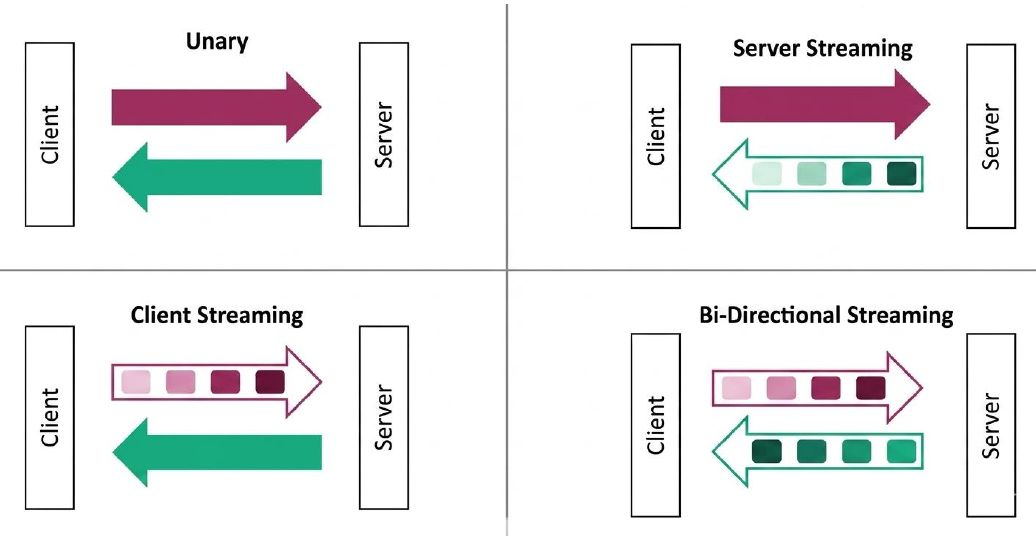
\includegraphics[scale=0.5]{figures/Schermata_20260515_104815.png}
\end{figure}

\subsection{File \texttt{.proto}}
Con gRPC non bisogna scrivere manualmente il codice per marshalling e unmarshalling.

\begin{enumerate}
    \item Si scrive un \textbf{file \texttt{.proto}}: definisce i \uline{messaggi (strutture dati) e i servizi (funzioni chiamabili remotamente)}.
    \item Il codice viene compilato per mezzo del \textbf{compilatore \texttt{gRPC}}
\end{enumerate}

\begin{figure}[H]
    \centering
    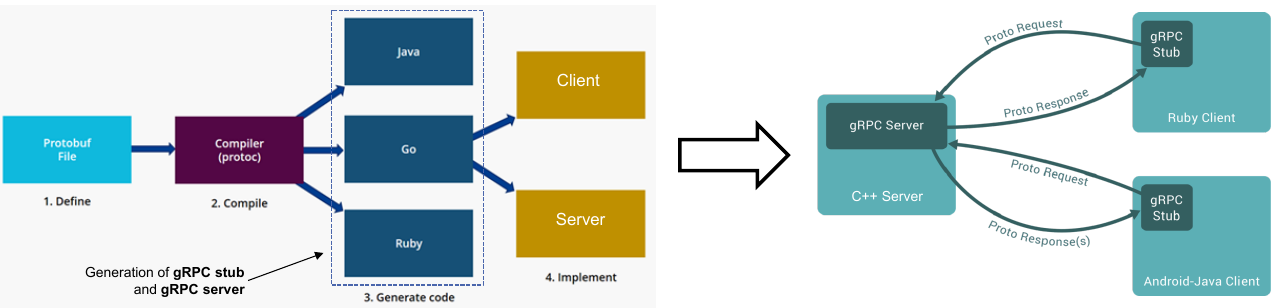
\includegraphics[scale=0.5]{figures/Schermata_20260515_105241.png}
\end{figure}

\begin{tcolorbox}[breakable, title={Esempio di file \texttt{.proto}}]
    Si vuole poter o chiedere lo stato attuale (Unary RPC) oppure ricevere aggiornamenti costanti (Streaming RPC)

    \begin{lstlisting}
// Specifica la versione della sintassi (proto3 e' lo standard attuale)
syntax = "proto3";

// Definizione dei messaggi: o i dati specificati dall'utente (SensorRequest) o creati dal sensore (EnvironmentData)
// I numeri (1, 2, 3) sono i "Tag", ovvero identificatori binari delle variabili usati in fase di comunicazione
message SensorRequest {
  int32 sensor_id = 1; // ID del sensore specifico
}

message EnvironmentData {
  float temperature = 1; // Temperatura
  float humidity = 2;    // Umidita' in percentuale
  string status = 3;     // Es. "OTTIMALE", "ALLERTA"
}

// Definizione del servizio: le procedure (funzioni) disponibili
service SystemMonitor {
  // 1. Unary RPC: Il client chiede i dati e riceve una sola risposta
  rpc GetCurrentStatus(SensorRequest) returns (EnvironmentData);

  // 2. Server Streaming: Il client chiede di monitorare e il server invia un flusso continuo di dati (es. ogni sec.)
  rpc WatchEnvironment(SensorRequest) returns (stream EnvironmentData);
}
    \end{lstlisting}
\end{tcolorbox}

\subsection{Timeout}
La chiamata viene annullata automaticamente dopo un certo tempo.
\subsection{Cancellazione della chiamata}
Viene inviata una notifica al server, il quale può smettere di lavorare.
\subsection{Autenticazione}
Supporto nativo (es. SSL/TLS)

\chapter{\texttt{Java RMI}}
\section{Definizione}
È un \texttt{middleware} che \uline{consente a oggetti su una \texttt{JVM} di accedere a o invocare un oggetto in esecuzione su un'altra \texttt{JVM}}.

È un implementazione di \texttt{RPC} che \textbf{permette la comunicazione remota tra programmi} Java trasparente al programmatore.

Viene fornito dal pacchetto \textbf{\texttt{java.rmi}}

\section{Architettura di un'applicazione RMI}
\subsection{Procedura}
Vengono scritti due programmi: un \textbf{programma client} e un \textbf{programma server}.
\begin{itemize}
    \item Nel \uline{programma server} viene creato un \textbf{oggetto remoto}.
    \item Un \textbf{riferimento} a tale oggetto \uline{viene messo a disposizione del client}.
    \item Il programma client richiede \textbf{l'accesso all'oggetto remoto} e cerca di \textbf{invocare i suoi metodi}
\end{itemize}
\subsection{Problematiche fondamentali}
\begin{itemize}
    \item Come passare i parametri a un oggetto?
    \item Come passare il riferimento remoto relativo a un oggetto?
    \item Nel caso di riferimento locale, come passare lo stato dell'oggetto?
    \item Nel caso di riferimento locale, come ricostruire la struttura dell'oggetto lato server?
\end{itemize}

\section{Ricostruzione dell'oggetto - \texttt{Java Runtime Enviroment}}
In Java il problema della ricostruzione della struttura dell'oggetto è risolvibile nativamente grazie al \texttt{Java Runtime Enviroment}.

Il \textbf{class loader} ha il compito di caricare le classi (file \texttt{.class}, formato bytecode)
\begin{itemize}
    \item I file \texttt{.class} possono essere trasferiti da librerie, file system locali o nodi remoti in rete.
    \item Il caricamento avviene dinamicamente quando
    \begin{itemize}
        \item Viene eseguito il comando \texttt{new}, oppure
        \item Un oggetto viene trasferito per mezzo di \texttt{RMI} (se il file \texttt{.class} non è presente localemnte).
    \end{itemize}
\end{itemize}

Il file \texttt{.class} include:
\begin{itemize}
    \item \textbf{Struttura e metadati della classe}.
    \item \textbf{Tabella dei simboli}.
    \item \textbf{Bytecode dei metodi}.
    \item \textbf{Definizione dei campi}.
\end{itemize}

\begin{figure}[H]
    \centering
    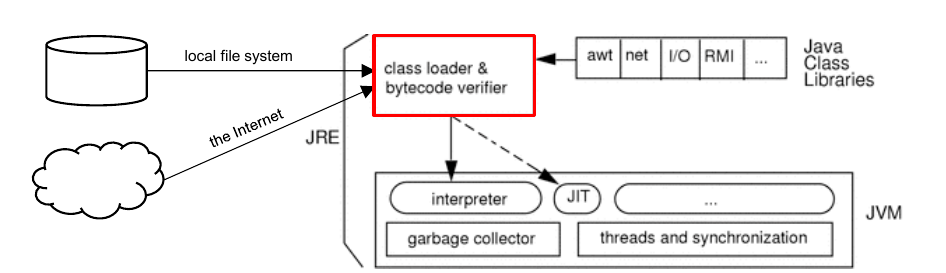
\includegraphics[scale=0.7]{figures/Schermata_20260515_114139.png}
\end{figure}

\section{Passaggio dei parametri}
\subsection{Passaggio per valore}
\begin{itemize}
    \item Tipi primitivi
    \item Oggetti non remoti, devono implementare l'interfaccia \texttt{java.io.Serializable}.
\end{itemize}
\subsection{Passaggio per riferimento}
Per passare oggetti remoti si utilizza la classe \texttt{java.rmi.server.UnicastRemoteObject} e serve per implementare
\subsubsection{\texttt{Java.io.Serializable}}
Specifica che l'oggetto è un "contenitore di dati" e che può essere somantato in una sequenza di byte, spedito in rete e rimontato
\begin{itemize}
    \item Passaggio per valore.
    \item Viene ricevuta una copia esatta dello \textbf{stato (variabili)} dell'oggetto originario.
\end{itemize}
\subsubsection{\texttt{java.rmi.Remote}}
Specifica che l'oggetto è remoto e i suoi metodi possono essere invocati da programmi eseguiti su altre macchine.
\begin{itemize}
    \item Se un oggetto che implementa \texttt{Remote} viene passato come parametro in una chiamata remota, non viene inviato l'oggetto vero e proprio ma il suo \textbf{stub}.
    
    Passaggio per riferimento.
    \item Lo stub è un oggetto includente il \textbf{riferimento}, ovvero:
    \begin{itemize}
        \item Indirizzo IP del server.
        \item Porca TCP del processo.
        \item Identificativo univoco dell'oggetto.àà
    \end{itemize}

    La classe \texttt{UnicastRemoteObject} implementa \texttt{Serializable} per permettere la serializzazione dello stub.
\end{itemize}

\section{Passaggio dello stato - Serializzazione dell'oggetto}
La serializzazione rappresenta lo stato di un oggetto come \textbf{stream di byte}, è essenziale per poter memorizzare e ricostruire lo \textbf{stato} degli oggetti.
\begin{itemize}
    \item Per definire oggetti persistenti.
    \item Per trasferire oggetti via rete.
\end{itemize}

Per mezzo della serializzazione devono essere passate solo le informazioni essenziali sullo stato, la descrizzione della classe (struttura) è caricata a parte (file \texttt{.class}).

\begin{itemize}
    \item La serializzazione usa il metodo \texttt{writeObject(Object obj)} della classe \texttt{ObjectOutputStream}
    \begin{itemize}
        \item Attraversa ricorsivamente tutti i riferimenti ad altri oggetti contenuti in \texttt{obj} per costruire una rappresentazione completa del \textbf{grafo degli oggetti}.
        \item Vengono serializzati tutti gli oggetti del grafo (devono implemetare \texttt{Serializable}).
    \end{itemize}

    Il processo inverso (deserializzazione) usa il metodo \texttt{readObject()}.
\end{itemize}

\begin{tcolorbox}[breakable, title={Esempio (oggetto persistente)}]
    \begin{lstlisting}[language=java]
// serializzazione di stringa e data odierna su un file
FileOutputStream f = new FileOutputStream("tmp"); // creazione canale di comunicazione per scrittura su file
ObjectOutputStream s1 = new ObjectOutputStream(f); // creazione oggetto per serializz.
s1.writeObject("Today"); // serializzazione stringa
s1.writeObject(new Date()); // serializzazione oggetto data
s1.flush(); // passaggio dei dati serializzati da buffer a file (quando buffer non pieno)

// deserializzazione di stringa e data da file
FileInputStream in = new FileInputStream("tmp"); //creazione canale di comunicazione per lettura da file
ObjectInputStream s2 = new ObjectInputStream(in); // creazione oggetto per deserializzazione
String today = (String)s2.readObject(); // deserializzazione stringa
Date date = (Date)s2.readObject(); // deserializzazione oggetto data
    \end{lstlisting}
\end{tcolorbox}

\section{Passaggio dei riferimenti}
RMI definisce un componente chiamato \textbf{\texttt{RMI registry}}
\begin{itemize}
    \item Si ha un \texttt{rmiregistry} su ogni macchina che ospita oggetti remoti.
    \item Associa univocamente un nome logico assegnato all'oggetto al suo riferimento.
    \item RMI attiva un servizio di ascolto per quel servizio.
\end{itemize}

Viene utilizzata la classe \texttt{java.rmi.Naming} per accedere alle funzionalità dell'\texttt{RMI registry}
\begin{itemize}
    \item Metodi fondamentali: \texttt{bind} e \texttt{lookup}.
\end{itemize}

\begin{figure}[H]
    \centering
    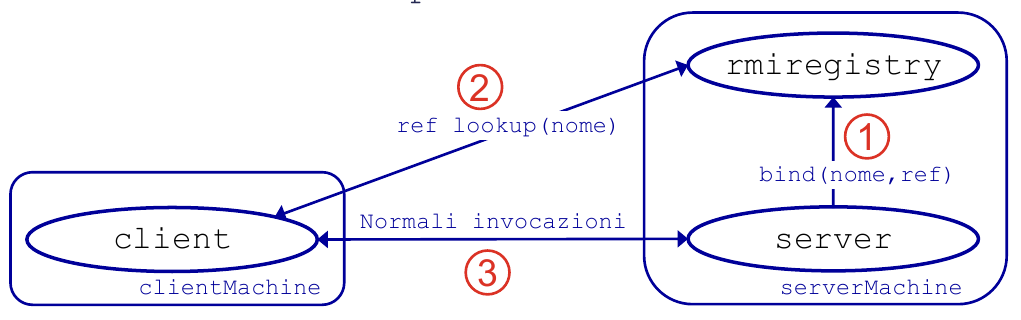
\includegraphics[scale=0.5]{figures/Schermata_20260515_115647.png}
\end{figure}
\subsection{La classe \texttt{java.rmi.Naming}}
\subsubsection{Parametri}
\begin{itemize}
    \item \texttt{name}: Nome logico dell'oggetto in formato URL.
    \item \texttt{obj}: Il riferimento all'oggetto remoto (solitamente un oggetto stub).
\end{itemize}
\subsubsection{Metodi}
\begin{itemize}
    \item \texttt{public static void bind(String name, Remote obj) throws AlreadyBoundException, MalformedURLException, RemoteException}
    \begin{itemize}
        \item Collega il nome specificato all'oggetto remoto
    \end{itemize}

    \item \texttt{public static void rebind(String name, Remote obj) throws RemoteException, MalformedURLException}
    \begin{itemize}
        \item Collega (bind) il nome specificato all'oggetto remoto, cancellando i collegamenti esistenti
    \end{itemize}

    \item \texttt{public static Remote lookup(String name) throws NotBoundException, MalformedURLException, RemoteException}
    \begin{itemize}
        \item Restituisce un riferimento (stub) all'oggetto associato al nome specificato
    \end{itemize}

    \item \texttt{public static String[] list(String name) throws RemoteException, MalformedURLException}
    \begin{itemize}
        \item Restituisce i nomi (in formato URL) degli oggetti del registry
    \end{itemize}

    \item \texttt{public static void unbind(String name) throws RemoteException, NotBoundException, MalformedURLException}
    \begin{itemize}
        \item Distrugge il collegamento (bind) al nome specifico
    \end{itemize}
\end{itemize}
\subsubsection{Eccezioni}
\begin{itemize}
    \item \texttt{AlreadyBoundException}: Il nome è già collegato a un altro oggetto.
    \item \texttt{NotBoundException}: Il nome non è collegato ad alcun oggetto.
    \item \texttt{RemoteException}: Il registry non può essere contattato.
    \item \texttt{MalformedURLException}: Il nome non è un RUL formattato in modo appropriato.
\end{itemize}

\subsection{Workflow in dettaglio}
\begin{enumerate}
    \item Il server pubblica il riferimento e il nome dell'oggetto remoto nel registry invocando il metodo \texttt{bind}.
    \item Il client ottiene il Server Stub e il riferimento all'oggetto remoto invocando il metodo \texttt{lookup}.
    \item Il client invoca il metodo sullo stub, il quale inoltra al server il riferimento dell'oggetto remoto e l'identificativo del metodo da eseguire, più i parametri del metodo.
    \item Il registry ha stub e skeleton $\to$ È un oggetto remoto con cui bisogna comunicare.
\end{enumerate}

\begin{figure}[H]
    \centering
    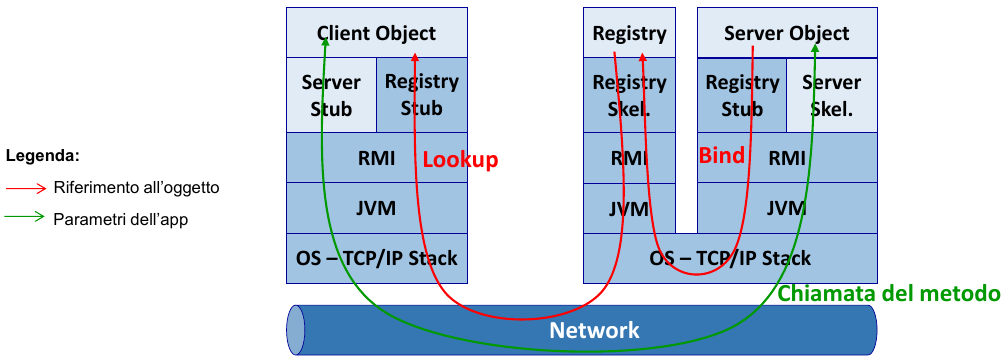
\includegraphics[scale=0.5]{figures/Schermata_20260515_121237.png}
\end{figure}


\section{Problematiche fondamentali dei sistemi distribuiti e Java RMI}
In che modo le problematiche fondamentali dei sistemi distribuiti sono affrontate quando \texttt{Java RMI} è adottato per l'invocazione di metodi di oggetti remoti?

\begin{enumerate}
    \item Identificazione della controparte (naming)

    Sono necessari l'hostname e il nome dell'oggetto.
    \item Accedere alla controparte (access point)

    Accesso per mezzo del \texttt{RMI registry}
    \item Comunicazione 1 (protocol)

    Serializzazione degli oggetti locali o riferimento a oggetti remoti.
    \item Comunicazione 2 (syntax and semantics)

    Tipi di Java
\end{enumerate}


\section{Vantaggi e Svantaggi}
\subsection{Vantaggi (rispetto a implementazioni \texttt{RPC} generali)}
\begin{itemize}
    \item Supporto nativo a un design orientato agli oggetti.
    \item Integrazione totale e trasparente con il linguaggio Java.
\end{itemize}
\subsection{Svantaggi (rispetto a implementazioni \texttt{RPC} generali)}
\begin{itemize}
    \item Legato indissolubilmente a Java.
    \item Overhead maggiore e prestazioni minori.
    \item Maggior complessità a livello di rete e problemi di sicurezza.
\end{itemize}